\section{Introduction}
\label{sec:introduction}
\outline{Use the classical Roofline~\cite{williams2009roofline} and Fig.~\ref{fig:operand-roles} to motivate separate accounting for establishing resident state and evaluating streaming inputs in compute-in-memory (CIM). Position the contribution relative to Jia et al.'s IMC write/compute analysis~\cite{jia2022imc}: their energy-efficiency view already exposes amortization, while this paper develops role- and window-based throughput accounting. Lead from the bound to the native capability map and reuse thresholds in Figs.~\ref{fig:hardware-capacities} and~\ref{fig:critical-reuse}, with inference matrix stages providing concrete demand examples.}
\draftreserve{1.20in}{Introduction: motivation, nearest prior work, and contribution.}
\draftcolumnbreak
% A true float in both modes: it must reach the top of the column beside the drafted Introduction.
\begin{figure}[!t]
\centering
% Fig1_cropped.png is generated from Fig1.png by crop_fig1.py.
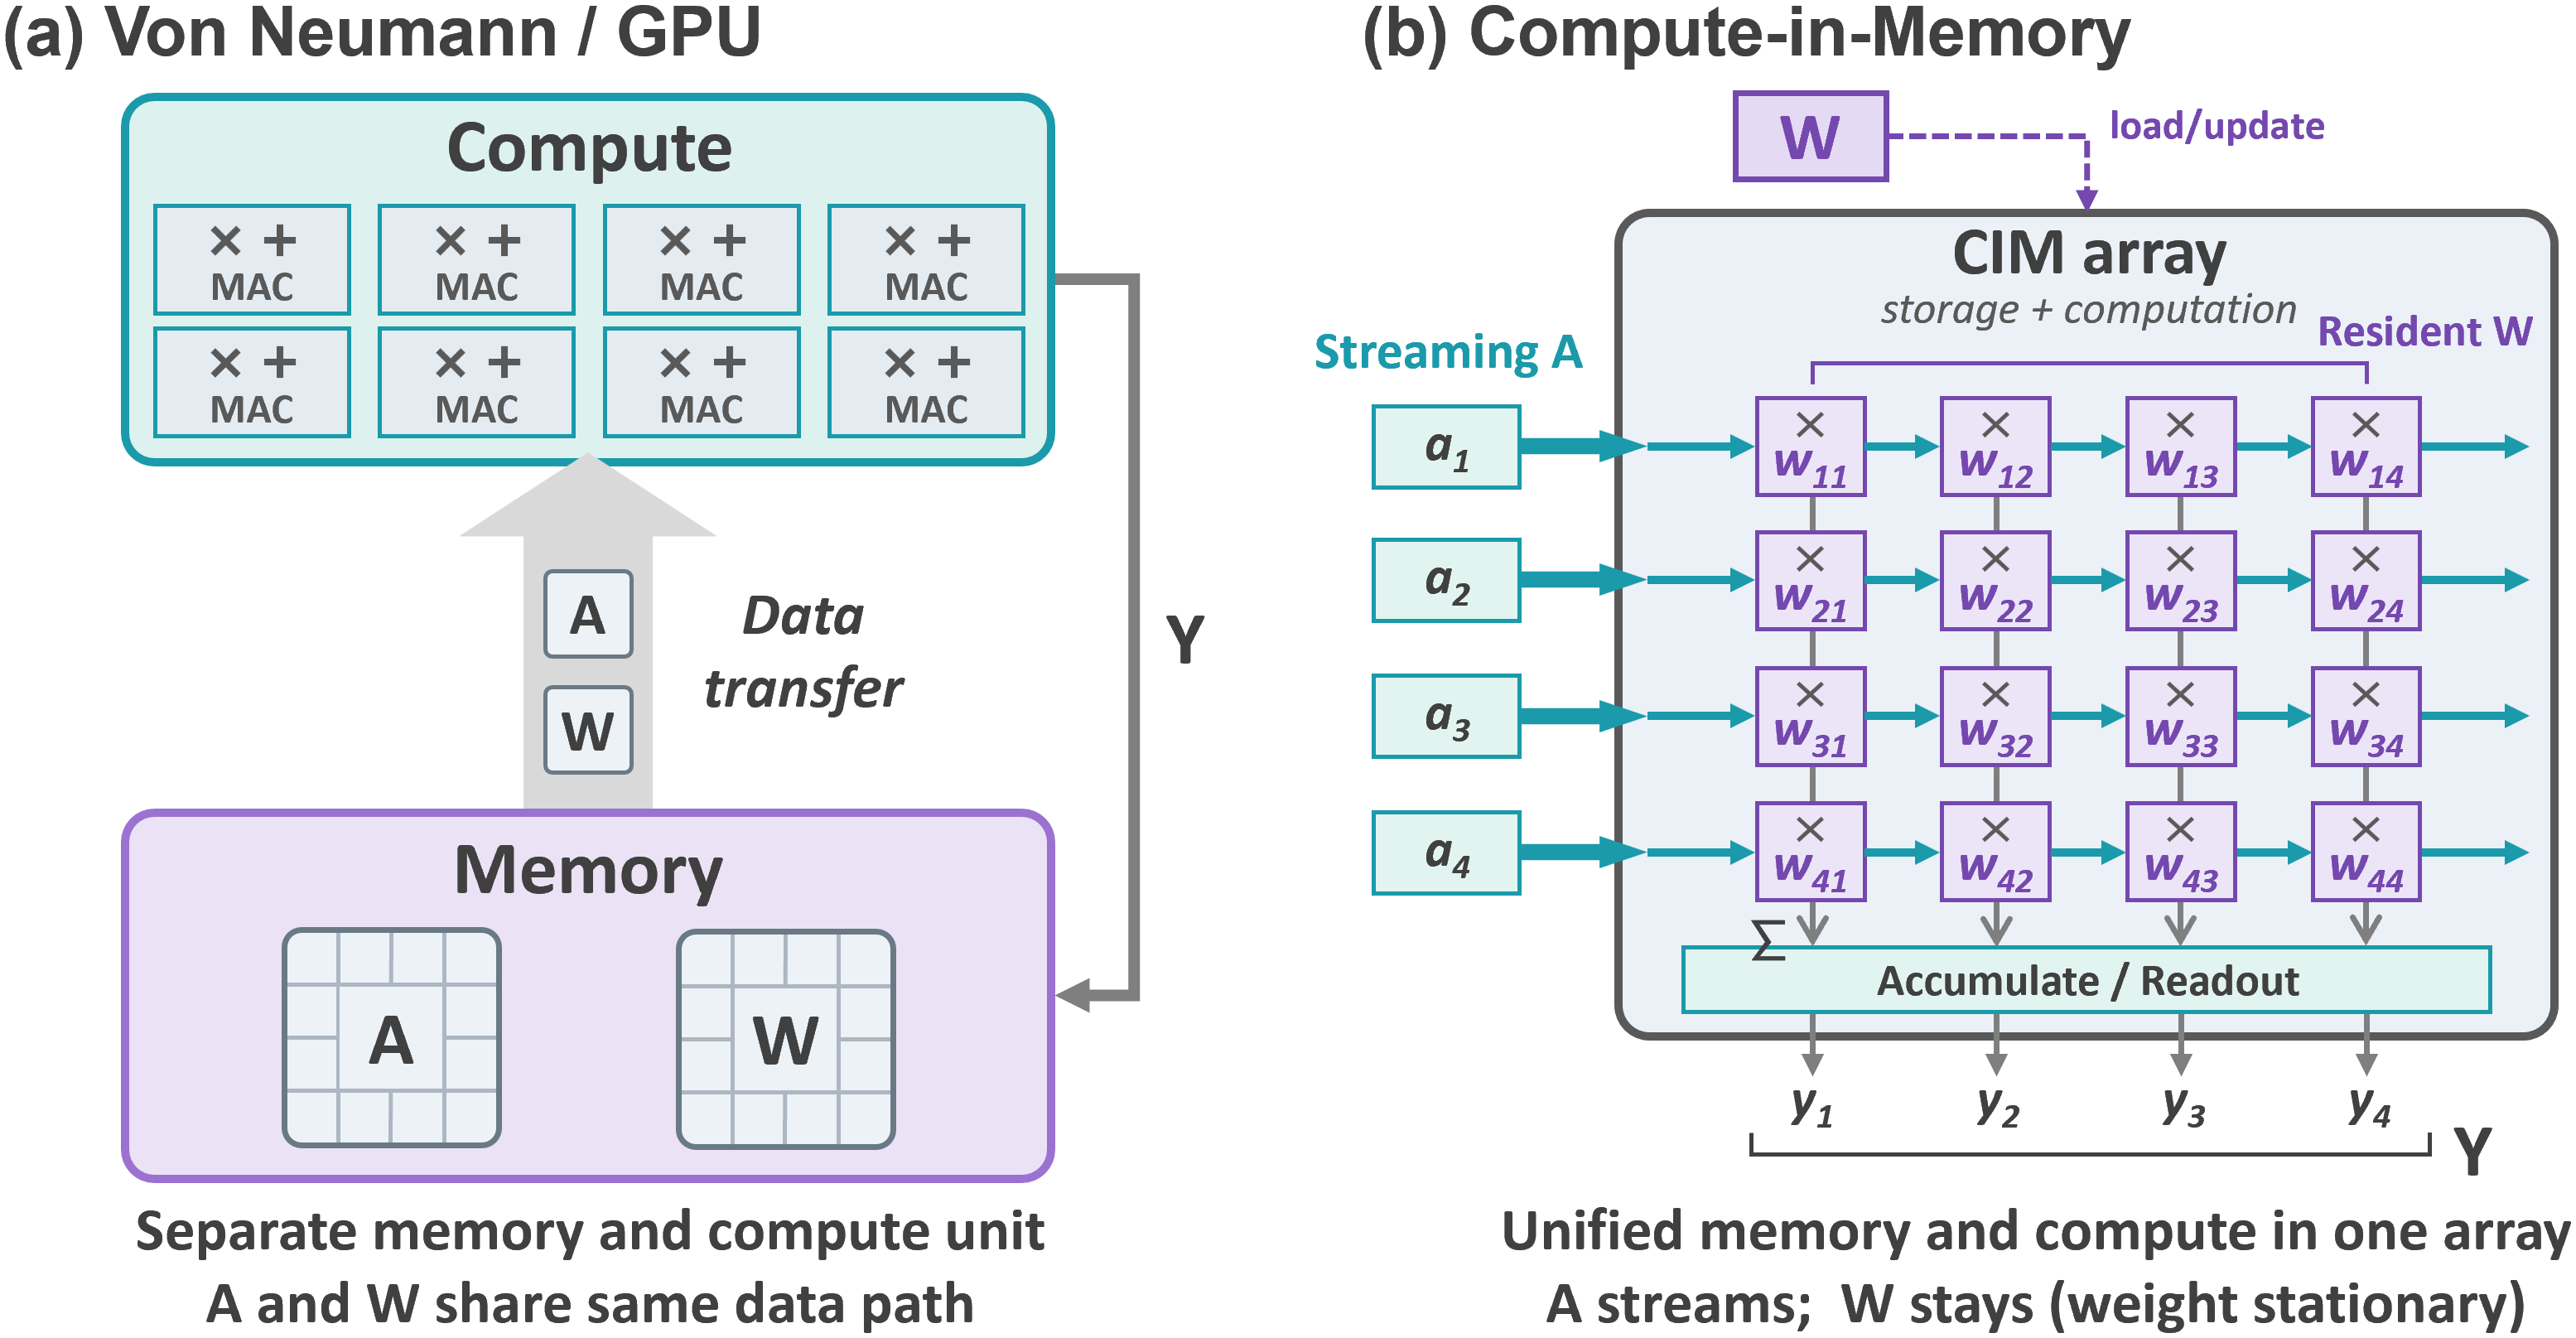
\includegraphics[width=\linewidth]{figures/Fig1_cropped.png}
\caption{Operand roles in (a) separate memory and compute units and (b) a CIM array. Streaming inputs $A$ are evaluated against resident weights $W$, with a distinct path for loading or updating $W$.}
\label{fig:operand-roles}
\vspace{-20pt}
\end{figure}

